\glsunset{if}\glsunset{im}\glsunset{af}\glsunset{am}\glsunset{bf}\glsunset{bm}\glsunset{wf}\glsunset{wm}
\section{The BFW Benchmark and Dataset}


We now discuss the \gls{bfw} dataset, and protocols to evaluate \gls{ml}-based \gls{fr}. We  conclude this section by reviewing the human evaluation conducted as part of this work, to detect bias in humans.

\subsection{The data}
Problems of bias in \gls{fr} motivated the design of \gls{bfw}. The data evenly represent various subgroups partitioned by demographics. Inspired by \gls{dp}~\cite{demogPairs}, the specification of \gls{bfw} follows in suit. \gls{bfw} includes additional subgroups (\ie \gls{if} and \gls{im}), an increased in the number subjects per subgroup, with many more pairs (Table~\ref{tab:ethnic-splits}). 




\vspace{1mm}
\noindent\textbf{Compiling subject list.} 
 All subjects were sampled from VGG2~\cite{Cao18}. Thus, unlike others that depend on multiple sources, \gls{bfw} has less potential conflicts in train/test overlap for existing models. We used pre-trained ethnicity~\cite{ambekar2009name} and gender~\cite{levi2015age} classifiers to find candidates for the different subgroups.



\vspace{1mm}
\noindent\textbf{Detecting faces.} Faces were detected using \gls{mtcnn}~\cite{zhang2016joint}.\footnote{\href{https://github.com/polarisZhao/mtcnn-pytorch}{https://github.com/polarisZhao/mtcnn-pytorch}} Then, assigned into one of two sets. Faces within detected bounding box (BB) regions extended out 130\% in each direction, with zero-padding as the boundary condition made-up one set. The second set were faces aligned and cropped for Arcface~\cite{deng2019arcface} (see the next step). Also, coordinates of the BB and the five landmarks per MTCNN were stored as part of the static, raw data. Samples with multiple face detections had the BB area times the confidence score of the MTCNN to determine the instance most likely to be the face, with others set aside and labeled \textit{miss-detection}. 

\begin{figure}[!t] 
	\centering    
 \glsunset{fpr}
  \glsunset{fnr}
	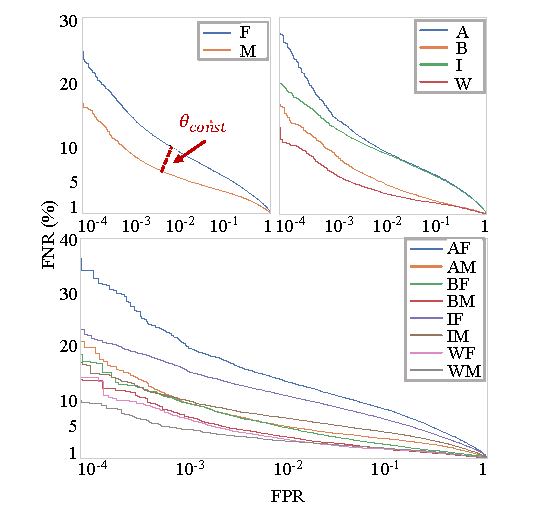
\includegraphics[trim=7mm 0.1in 5mm 0in,clip,width=\linewidth]{images/detcurve-improved.pdf}
		\caption{\textbf{\gls{det} curves.} \emph{Top-left}: per gender. \emph{Top-right}: per ethnicity. \emph{Bottom}: per subgroup (\ie combined). A dashed lined shows a difference by about 2$\times$ in \gls{fpr} for the same threshold $\theta_{const}$. \gls{fnr} is the number of match errors, so closer a curve is to the bottom better.}
		\glsreset{det}\glsreset{fpr}
\label{fig:detcurves} 
\vspace{-5mm}
\end{figure} 

\vspace{1mm}
\noindent\textbf{Validating labels.} 
Faces of \gls{bfw} were encoded using the original implementation of the \gls{soa} Arcface~\cite{deng2019arcface}. A matrix of cosine similarity scores was then generated for each subject, and removed samples (\ie rows) with median scores below threshold $\theta=0.2$. Mathematically, the $j^{th}$ subject with $N_j$ faces is removed if the ordinal rank of its score $n = \frac{P\times N}{100}\geq\theta$, with the percentile $P=50$, $\theta=0.2$ set manually, and an ordered list of scores. This allowed us to quickly prune \gls{fp} face detections. Following~\cite{robinson2016families, robinson2018visual}, we built a JAVA tool to visually validate the remaining faces. The faces were first ordered from most-to-least confidence, with confidence set as the average score, and then displayed as image icons on top toggling buttons arranged as a grid in a sliding pane window. Labeling then consisted of going subject-by-subject and flagging faces of \emph{imposters}. 
% Each subject underwent two passes by different annotators.

%  by flagging \emph{imposters}



\vspace{1mm}
\noindent\textbf{Sampling faces and creating folds.} We created lists of pairs in five-folds with subjects split evenly per subject and without overlap across folds. Furthermore, balance in the number of faces per was obtained by sampling twenty-five faces at random from each. Next, we generated a list of all face pairs per subject, resulting in $\sum_{l=1}^{L}\sum_{k=1}^{K_d} {N_k \choose 2}$ positive pairs, where the number of faces of all $K_l$ subjects $N_k=25$  for each of the $L$ subgroups (Table~\ref{tab:ethnic-splits}). Next, we assigned subjects to a fold. To preserve balance across folds, we sorted subjects by the number of pairs and then started assigning to alternating folds from the one with the most samples. Note, this left no overlap in identity between folds. Later, a negative set from samples within the same subgroup randomly matched until the count met that of the positive. Finally, we doubled the total count with negative pairs from across subgroups but in the same fold.
\begin{figure}[t!] 
	\glsunset{fpr}
	\centering
	\centering
	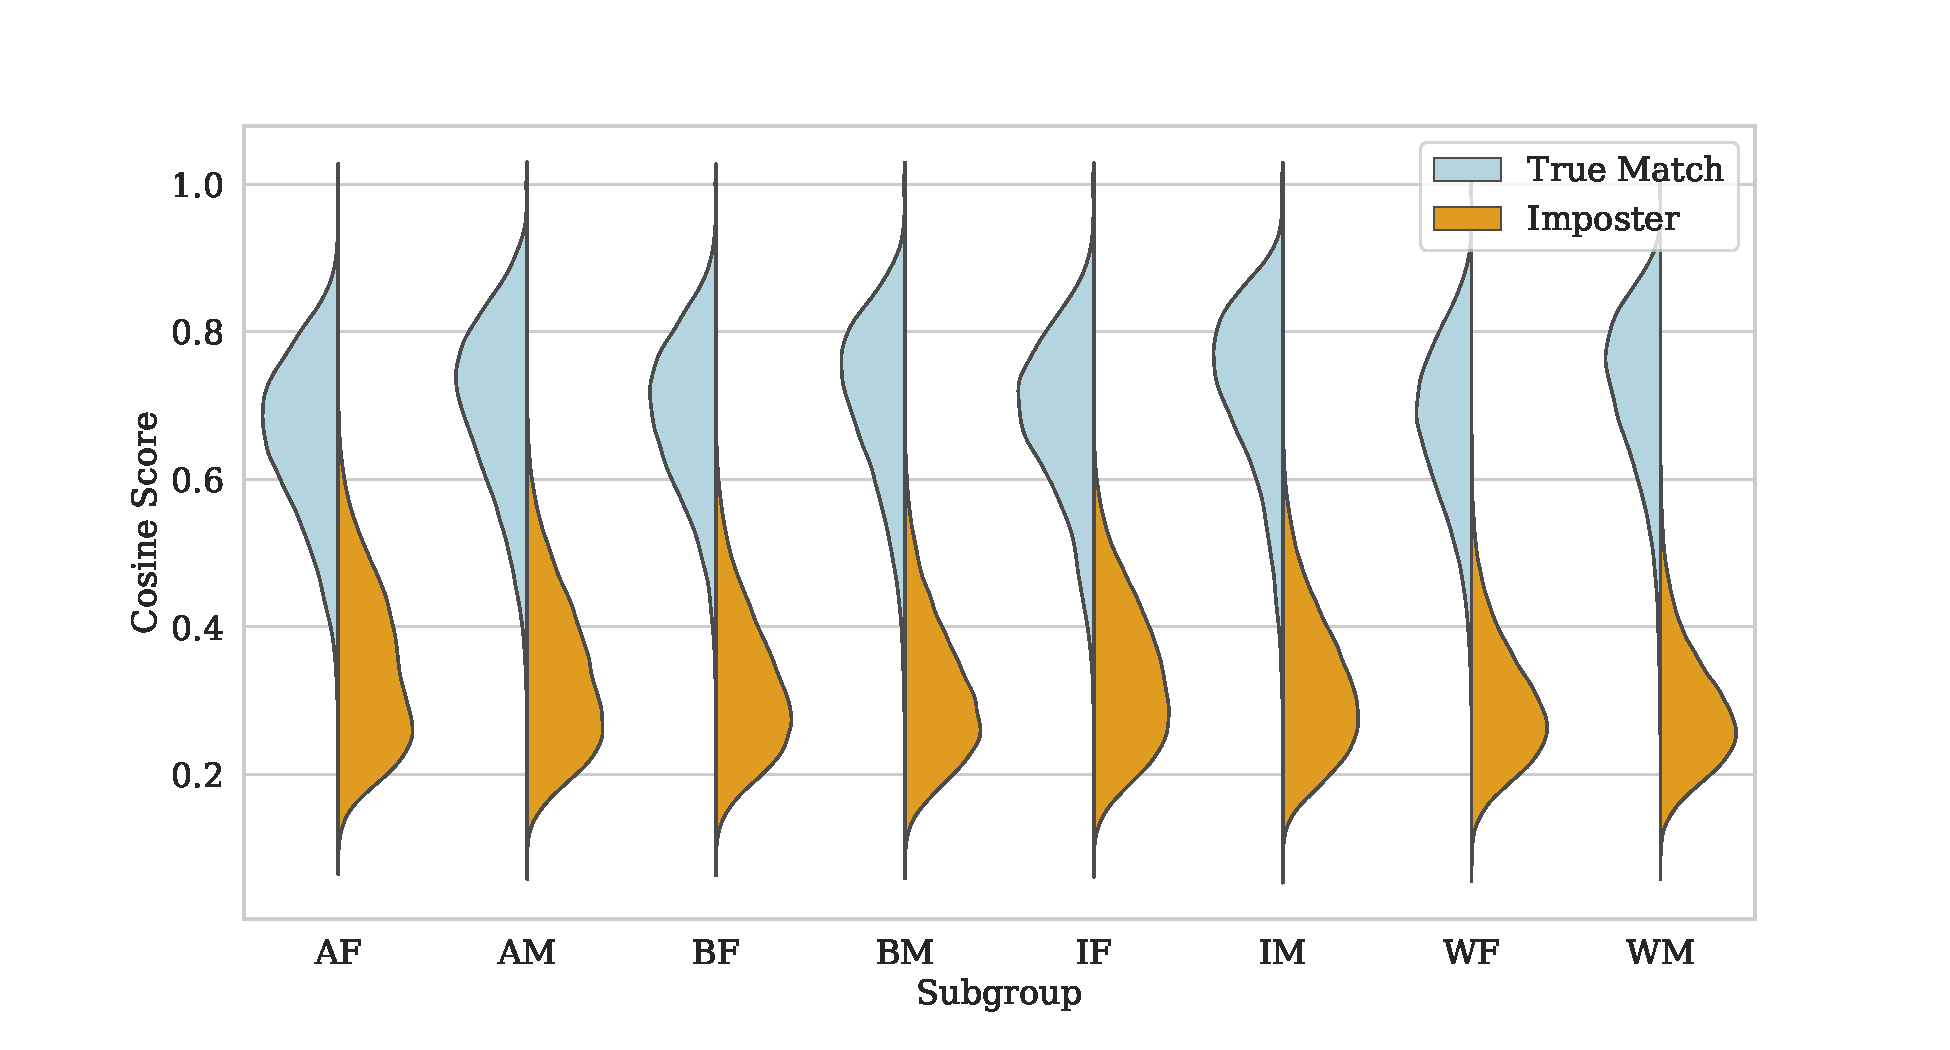
\includegraphics[trim=0.3in 0.1in 0.2in 0.2in,clip,angle=-0,origin=c,width=1\linewidth]{images/violinplots.pdf}
		\caption{\textbf{\Gls{sdm} across subgroups.} The scores for \emph{imposters} have medians about 0.3 but with variation in upper percentiles, while \emph{genuine} pairs vary in both (\eg \gls{af} has more area of overlap). A varying threshold varying across different subgroups yields a constant \gls{fpr}.} \label{fig:detection-model} 
\end{figure} 


\vspace{-5pt}
\subsection{Problem formulation}\label{subsec:pf} 
% \gls{lfw}~\cite{LFWTech}, a commonly used benchmark for ~\gls{fr}, reserves specific train-test face-pair lists. 
\Gls{fv} is the special case of the two-class (\ie boolean) classification. Hence, pairs are labeled as the ``same'' or ``different'' \textit{genuine} pairs (\ie \textit{match}) or \textit{imposter} (\ie \textit{mismatch}), respectfully. This formulation (\ie \gls{fv}) is highly practical for applications like access control, re-identification, and surveillance. Typically, training a separate model for each unique subjects is infeasible. Firstly, the computational costs compound as the number of subjects increase.  Secondly, such a scheme would require model retraining each time a new person is added. Instead, we train models to encode facial images in a feature space that captures the uniqueness of a face, to then determine the outcome based on the output of a scoring (or distance) function. Formally put:
\begin{equation}\label{eg:matcher}
    f_{boolean}(\vec{x}_i, \vec{x}_j) = d(\vec{x}_i, \vec{x}_j) \leq \theta
\end{equation}

where $f_{boolean}$ is the \textit{matcher} of the feature vector $\vec{x}$ for the $i^{th}$ and $j^{th}$ sample~\cite{LFWTech}.

Cosine similarity is used as the \emph{matcher} in Eq~\ref{eg:matcher} the closeness of $i^{th}$ and $j^{th}$ features, \ie
$
s_l= \frac{f_i\cdot f_j}{||f_i||_2||f_j||_2}
$ is the closeness of the $l^{th}$ pair. 


\subsection{Human Assessment}\label{subsec:human-assessment}
We evaluated human on face pairs focusing on two racial groups: Chinese and Caucasians. To focus on the experiment, we honed-in on two groups, white Americans (W) and Chinese from China (C). The purpose was to the minimize variability by only analyzing the subsets of the broader groups of whites and Asians. 

Samples were collected by recruiting subjects from multiple sources (\eg social media, email lists, and family/friends)-- a total of 120 participants were sampled at random from all the submissions that were (1) complete and (2) from a W or C participant. Specifically, there were 60 W and 60 C, both with \gls{m} and \gls{f} split evenly. A total of 50 face pairs of non-famous ``look-alikes'' were collected from the internet, with 20 ({\emph WA}) and 20 ({\emph C}) pairs (male and female split evenly). The other 10 pairs are of others (\eg Hispanic/ Latino, Japanese, African). Survey was created, distributed, and recorded via \href{https://paperform.co}{PaperForm}. 